\documentclass[bachelor, och, coursework]{SCWorks}
% параметр - тип обучения - одно из значений:
%    spec     - специальность
%    bachelor - бакалавриат (по умолчанию)
%    master   - магистратура
% параметр - форма обучения - одно из значений:
%    och   - очное (по умолчанию)
%    zaoch - заочное
% параметр - тип работы - одно из значений:
%    referat    - реферат
%    coursework - курсовая работа (по умолчанию)
%    diploma    - дипломная работа
%    pract      - отчет по практике
% параметр - включение шрифта
%    times    - включение шрифта Times New Roman (если установлен)
%               по умолчанию выключен
\usepackage{subfigure}
\usepackage{tikz,pgfplots}
\pgfplotsset{compat=1.5}
\usepackage{float}

%\usepackage{titlesec}
\setcounter{secnumdepth}{4}
%\titleformat{\paragraph}
%{\normalfont\normalsize}{\theparagraph}{1em}{}
%\titlespacing*{\paragraph}
%{35.5pt}{3.25ex plus 1ex minus .2ex}{1.5ex plus .2ex}

\titleformat{\paragraph}[block]
{\hspace{1.25cm}\normalfont}
{\theparagraph}{1ex}{}
\titlespacing{\paragraph}
{0cm}{2ex plus 1ex minus .2ex}{.4ex plus.2ex}

% --------------------------------------------------------------------------%
\usepackage[T2A]{fontenc}
\usepackage[utf8]{inputenc}
\usepackage{graphicx}
\graphicspath{ {./img/} }
\usepackage{tempora}

\usepackage[sort,compress]{cite}
\usepackage{amsmath}
\usepackage{amssymb}
\usepackage{amsthm}
\usepackage{fancyvrb}
\usepackage{listings}
\usepackage{listingsutf8}
\usepackage{longtable}
\usepackage{array}
\usepackage[english,russian]{babel}

\usepackage{url}
\usepackage[colorlinks=true, linkcolor=black]{hyperref}

\usepackage{underscore}
\usepackage{setspace}
\usepackage{indentfirst} 
\usepackage{mathtools}
\usepackage{amsfonts}
\usepackage{enumitem}
\usepackage{tikz}
\usepackage{textgreek}

\usepackage{minted}
\setminted[python3]{style=bw, linenos, breaklines=true, fontsize=\footnotesize}
\setminted[py]{fontsize=\small, breaklines=true, style=bw, linenos}

\newcommand{\eqdef}{\stackrel {\rm def}{=}}
\newcommand{\specialcell}[2][c]{%
\begin{tabular}[#1]{@{}c@{}}#2\end{tabular}}

\renewcommand\theFancyVerbLine{\small\arabic{FancyVerbLine}}

\newtheorem{lem}{Лемма}

\begin{document}

% Кафедра (в родительном падеже)
\chair{теоретических основ компьютерной безопасности и криптографии}

% Тема работы
\title{Обнаружение сетевого P2P-трафика}

% Курс
\course{4}

% Группа
\group{431}

% Факультет (в родительном падеже) (по умолчанию "факультета КНиИТ")
\department{факультета КНиИТ}

% Специальность/направление код - наименование
%\napravlenie{09.03.04 "--- Программная инженерия}
%\napravlenie{010500 "--- Математическое обеспечение и администрирование информационных систем}
%\napravlenie{230100 "--- Информатика и вычислительная техника}
%\napravlenie{231000 "--- Программная инженерия}
\napravlenie{10.05.01 "--- Компьютерная безопасность}

% Для студентки. Для работы студента следующая команда не нужна.
% \studenttitle{Студентки}

% Фамилия, имя, отчество в родительном падеже
\author{Стаина Романа Игоревича}

% Заведующий кафедрой
\chtitle{д. ф.-м. н., доцент} % степень, звание
\chname{М.~Б.~Абросимов}

%Научный руководитель (для реферата преподаватель проверяющий работу)
\satitle{д. к.ю. н., доцент} %должность, степень, звание
\saname{А.~В.~Гортинский}

% Руководитель практики от организации (только для практики,
% для остальных типов работ не используется)
% \patitle{к.ф.-м.н.}
% \paname{С.~В.~Миронов}

% Семестр (только для практики, для остальных
% типов работ не используется)
%\term{8}

% Наименование практики (только для практики, для остальных
% типов работ не используется)
%\practtype{преддипломная}

% Продолжительность практики (количество недель) (только для практики,
% для остальных типов работ не используется)
%\duration{4}

% Даты начала и окончания практики (только для практики, для остальных
% типов работ не используется)
%\practStart{30.04.2019}
%\practFinish{27.05.2019}

% Год выполнения отчета
\date{2023}

\maketitle

% Включение нумерации рисунков, формул и таблиц по разделам
% (по умолчанию - нумерация сквозная)
% (допускается оба вида нумерации)
% \secNumbering

%-------------------------------------------------------------------------------------------

% \begin{minted}[fontsize=\small]{MySQL}
% \end{minted}

% \begin{figure}[H]
%     \centering
%     \includegraphics[width=0.999\textwidth]{img/}
%     \caption{}
%     \label{easy_hack}
% \end{figure}

\tableofcontents

\intro
С развитием Интернета развивались файлообменные сети, благодаря которым появилась \textbf{P2P} (\textbf{p}eer-\textbf{to}-\textbf{p}eer) "--- одноранговая, децентрализованная или пиринговая сеть. Это распределённая архитектура приложения, которая разделяет задачи между узлами (peer). Узлы имеют одинаковые привилегии в приложении и образуют сеть равносильных узлов.

Узлы делают свои ресурсы, такие как вычислительная мощность, объем диска или пропускная способность, напрямую доступными остальным членам сети, без необходимости координировать действия с помощью серверов. Узлы являются одновременно поставщиками и потребителями ресурсов, в отличие от стандартной клиент-сервер модели, где поставщик и потребитель ресурсов разделены. \cite{P2P_1} 

В мае 1999 года, в Интернет с более чем миллионом пользователей, Шон Фэннинг внедрил приложение файлообменник Napster. 
Napster стал началом P2P-сети, такой какую мы знаем её сейчас, пользователи участвуют в создании виртуальной сети, 
полностью независимой от физической, без администрирования и каких-либо ограничений.

Концепция вдохновила новую философию во многих областях человеческого взаимодействия. 
P2P-технология позволяет пользователям интернета образовывать группы и коллаборации, формируя, тем самым, пользовательские поисковые движки, виртуальные суперкомпьютеры и файловые системы. 
Видение Всемирной паутины Тима Бернерса-Ли было близко к P2P-сети, в том смысле, 
что каждый пользователь является активным создателем и редактором контента.

В тоже время с появлением P2P появилась необходимость обнаруживать соотвествующий трафик в сети.
Универсального способа обнаружения работающего P2P-приложения нет. С развитием файлообменных сетей стало затруднительно
идентифицировать P2P-трафик с помощью номеров портов. Появилась необходимость исследования трафика на основании поведения узлов сети. Однако даже поведение такого трафика, его сигнатура и прочие признаки также могут изменяться со временем, поэтому все существующие методы должны обновляться и усовершенствоваться, чтобы поспевать за развитием P2P-приложений.

\section{Архитектура} 
P2P-сеть строится вокруг понятия равноправных узлов "--- клиенты и серверы одинаково взаимодействуют с другими узлами сети. 
Такая модель построения сети отличается от модели клиент-сервер, где взаимодействие идет с центральным сервером. 
На рисунке \ref{image1} а) изображены архитектура клиент-сервера и б) архитектура P2P. 
Типичным примером передачи файла в модели клиент-сервер является File Transfer Protocol (FTP), 
в котором программы клиента и сервера разделены: клиент инициирует передачу, а сервер отвечает на запросы. 

\begin{figure}[h]
    \begin{minipage}[h]{0.49\linewidth}
        \center{\includegraphics[width=0.75\linewidth]{arch_client-server.png} \\ а)}
    \end{minipage}
    \hfill
    \begin{minipage}[h]{0.49\linewidth}
        \center{\includegraphics[width=0.75\linewidth]{arch_p2p.png} \\ б)}
    \end{minipage}
    \caption{Архитектура клиент-сервера и P2P}
    \label{image1}
\end{figure}

\subsection{Базовые элементы P2P-сетей}
\subsubsection{Узел P2P-сети}
\textbf{Узел (Peer)} "--- фундаментальный составляющий блок любой одноранговой сети. 
Каждый узел имеет уникальный идентификатор и принадлежит одной или нескольким группам. 
Он может взаимодействовать с другими узлами как в своей, так и в других группах. \cite{P2P_2}

Виды узлов:
\begin{itemize}
    \item \textbf{Простой узел}. Обеспечивает работу конечного пользователя, предоставляя ему сервисы других узлов и	
    обеспечивая предоставление ресурсов пользовательского компьютера другим	участникам сети.
    \item \textbf{Роутер}. Обеспечивает механизм взаимодействия между узлами, отделёнными от сети брандмауэрами или NAT-системами.	
\end{itemize}

\subsubsection{Группа узлов}
\textbf{Группа узлов} "--- набор узлов, сформированный для решения общей задачи или достижения общей цели. 
Могут предоставлять членам своей группы такие наборы сервисов, которые недоступны узлам, входящим в другие группы.

Группы узлов могут разделяться по следующим признакам:
\begin{itemize}
    \item приложение, ради которого они объединены в группу;
    \item требования безопасности;
    \item необходимость информации о статусе членов группы.
\end{itemize}

\subsubsection{Сетевой транспорт}
\textbf{Конечные точки (Endpoints)} "--- источники и приёмники любого массива данных передаваемых по сети.

\textbf{Пайпы (Pipes)} "--- однонаправленные, асинхронные виртуальные коммуникационные каналы, соединяющие две или более конечные точки.

\textbf{Сообщения} "--- контейнеры информации, которая передаётся через пайп от одной конечной точки до другой.

\subsection{Маршрутизация}
P2P относят к прикладному уровню сетевых протоколов, а P2P-сети обычно реализуют некоторую форму виртуальной (логической) сети, наложенной поверх физической, то есть описывающей реальное расположение
и связи между узлами, такой сети, где узлы образуют подмножество узлов в физической сети. 
Данные по-прежнему обмениваются непосредственно над базовой TCP/IP сетью, 
а на прикладном уровне узлы имеют возможность взаимодействовать друг с другом напрямую, 
с помощью логических связей. Наложение используется для индексации и обнаружения узлов, 
что позволяет системе P2P быть независимой от физической сети. На основании того, как узлы соединены 
друг с другом внутри сети, и как ресурсы индексированы и расположены, сети классифицируются на 
\textbf{неструктурированные} и \textbf{структурированные} (или как их \textbf{гибрид}).

\subsubsection{Неструктурированные сети}
Неструктурированная Р2Р сеть не формирует определенную структуру сети, а случайным образом соединяет узлы друг с другом. 
Неструктурированные сети легко организуются и доступны для локальных оптимизаций, так как не существует глобальной структуры формирования сети.
Кроме того, поскольку роль всех узлов в сети одинакова, неструктурированные сети являются весьма надежными в условиях, 
когда большое количество узлов часто подключаются к сети или отключаются от неё.

Однако из-за отсутствия структуры возникают некоторые ограничения. 
В частности, когда узел хочет найти нужный фрагмент данных в сети, поисковый запрос должен быть направлен через сеть, 
чтобы найти как можно больше узлов, которые обмениваются данными. Такой запрос вызывает очень высокое количество сигнального трафика в сети, 
требует высокой производительности и не гарантирует, что поисковые запросы всегда будут решены.

\subsubsection{Структурированные сети}
В структурированных Р2Р-сетях наложение организуется в определенную топологию, и протокол гарантирует, 
что любой узел может эффективно участвовать в поиске файла или ресурса, даже если ресурс использовался крайне редко.

Наиболее распространенный тип структурированных сетей P2P реализуется распределенными хэш-таблицами (DHT), 
в котором последовательное хеширование используется для привязки каждого файла к конкретному узлу. Это позволяет узлам искать ресурсы в сети, используя хэш-таблицы, хранящие пару ключ-значение, и любой участвующий узел может эффективно извлекать значение, связанное с заданным ключом.

Тем не менее, для эффективной маршрутизации трафика через сеть, узлы структурированной сети должны обладать списком соседей, которые удовлетворяют определенным критериям. 
Это делает их менее надежными в сетях с высоким уровнем оттока абонентов (т.е. с большим количеством узлов, 
часто подключающихся к сети или отключающихся от нее).

\subsubsection{Гибридные модели}
Гибридные модели представляют собой сочетание Р2Р-сети и модели клиент-сервер. 
Гибридная модель должна иметь центральный сервер, который помогает узлам находить друг друга. 
Есть целый ряд гибридных моделей, которые находят компромисс между функциональностью, обеспечиваемой структурированной сетью модели клиент-сервер, 
и равенством узлов, обеспечиваемым чистыми одноранговыми неструктурированными сетями. 
В настоящее время гибридные модели имеют более высокую производительность, чем чисто неструктурированные или чисто структурированные сети.

\subsection{Безопасность}
Как и любая другая форма программного обеспечения, P2P-приложения могут содержать уязвимости. 
Особенно опасным для P2P программного обеспечения, является то, что Р2Р-приложения действуют и в качестве серверов, и в качестве клиентов, а это означает, что они могут быть более уязвимы для удаленных эксплоитов.

\subsubsection{Маршрутизационные атаки}
Поскольку каждый узел играет роль в маршрутизации трафика через сеть, злоумышленники могут выполнять различные <<маршрутизационные атаки>> или атаки отказа в обслуживании. Примеры распространенных атак маршрутизации включают в себя <<неправильную маршрутизацию поиска>>, когда вредоносные узлы преднамеренно пересылают запросы неправильно или возвращают ложные результаты, <<неправильную маршрутизацию обновления>>, когда вредоносные узлы изменяют таблицы маршрутизации соседних узлов, посылая им ложную информацию, и <<неправильную маршрутизацию разделения сети>>, когда новые узлы подключаются через вредоносный узел, который помещает новичков в разделе сети, заполненной другими вредоносными узлами.

\subsubsection{Поврежденные данные и вредоносные программы}
Распространенность вредоносных программ варьируется между различными протоколами одноранговых сетей. 
Исследования, анализирующие распространение вредоносных программ по сети P2P, обнаружили, например, что 63\% запросов на загрузку по сети Limewire содержали некоторую форму вредоносных программ, в то время как на OpenFT только 3\% запросов содержали вредоносное программное обеспечение. Другое исследование анализа трафика в сети Kazaa показало, что 15\% от 500 000 отобранных файлов были инфицированы одним или несколькими из 365 различных компьютерных вирусов.

Поврежденные данные также могут быть распределены по P2P-сети путем изменения файлов, которые уже были в сети. 
Например, в сети FastTrack, RIAA удалось внедрить фальшивые данные в текущий список загрузок и в уже загруженные файлы (в основном файлы MP3). 
Файлы, инфицированные вирусом RIAA, были непригодны впоследствии и содержали вредоносный код. 
Следовательно, P2P-сети сегодня внедрили огромное количество механизмов безопасности и проверки файлов. 
Современное хеширование, проверка данных и различные методы шифрования сделали большинство сетей устойчивыми к 
практически любому типу атак, даже когда основные части соответствующей сети были заменены фальшивыми или нефункциональными узлами.

\subsection{Отказоустойчивость и масштабируемость сети}
Децентрализованность Р2Р-сетей повышает их надежность, так как этот метод взаимодействия устраняет ошибку единой точки разрыва, присущую клиент-серверным моделям. С ростом числа узлов объем трафика внутри системы увеличивается, масштаб сети так же увеличивается, что приводит к уменьшению вероятности отказа. Если один узел перестанет функционировать должным образом, то система в целом все равно продолжит работу. 
В модели клиент-сервер с ростом количества пользователей уменьшается количество ресурсов выделяемых на одного пользователя, что приводит к риску возникновения ошибок.

\subsection{Распределенное хранение и поиск}
Возможность резервного копирования данных, восстановление и доступность приводят как к преимуществам, так и к недостаткам Р2Р-сетей. 
В централизованной сети только системный администратор контролирует доступность файлов. 
Если администраторы решили больше не распространять файл, его достаточно удалить с серверов,
и файл перестанет быть доступным для пользователей. Другими словами, клиент-серверные модели имеют возможность управлять доступностью файлов. В Р2Р-сети доступность контента определяется степенью его популярности, так как поиск идет по всем узлам, через которые файл проходил. 
То есть, в Р2Р-сетях нет централизованного управления как системного администратора в клиент-серверном варианте, 
а сами пользователи определяют уровень доступности файла.

\section{Применение P2P}
В Р2Р сетях, пользователи передают и используют контент сети. Это означает, что, в отличие от клиент-серверных сетей, 
скорость доступа к данным возрастает с увеличением числа пользователей, использующих этот контент. 
На этой идее построен протокол BitTorrent "--- пользователи, скачавшие файл, становятся узлами и помогают другим пользователям скачать файл быстрее. 
Эта особенность является главным преимуществом Р2Р сетей.

Множество файлообменных систем, таких как Gnutella, G2 и eDonkey популяризовали Р2Р технологии:
\begin{itemize}
    \item Пиринговые системы распространения контента.
    \item Пиринговые системы обслуживания, например, повышение производительности, в частности, Correli Caches.
    \item Пиринговые платёжные системы.
    \item Публикация и распространение программного обеспечения (Linux, видеоигры).
    \item Аудио- и видео-звонки.
\end{itemize}

В связи децентрализованностью доступа к данным в Р2Р сетях возникает проблема нарушения авторских прав. 
Компании, занимающиеся разработкой Р2Р приложений часто принимают участие в судебных конфликтах. 
Самые известные судебные дела это Grokster против RIAA и MGM Studios, Inc. против Grokster Ltd., 
где в обоих случаях технологии файлообменных систем признавались законными.

\section{Обнаружение P2P трафика без анализа полезной нагрузки}
\subsection{Анализ портов}
Многие P2P-приложения работают на определённых портах. 
Некоторые из таких указаны в таблице \ref{table:p2p-ports} \cite{p2p-list}.

\begin{table}[H]
    \caption{Список наиболее известных портов, используемых P2P-протоколами}
    \label{table:p2p-ports}
    \begin{center}
    {\small
    \begin{tabular}{|c|c|c|c|c|c|c|c|c|}
        \hline
    Протоколы   & Номера TCP/UDP портов \\ \hline
    BitTorrent      & 6881-6999  \\ \hline
    Direct Connect  & 411, 412, 1025-32000  \\ \hline
    eDonkey         & 2323, 3306, 4242, 4500, 4501, 4661-4674, 4677, 4678, 4711, 4712  \\ \hline
    FastTrack       & 1214, 1215, 1331, 1337, 1683, 4329  \\ \hline
    Yahoo           & 5000-50010, 5050, 5100  \\ \hline
    Napster         & 5555, 6257, 6666, 6677, 6688, 6699-6701  \\ \hline
    MSN             & 1863, 6891-6901 \\ \hline
    MP2P            & 10240-20480, 22321, 41170  \\ \hline
    Kazaa           & 1214  \\ \hline
    Gnutella        & 6346, 6347  \\ \hline
    ARES Galaxy     & 32285  \\ \hline
    AIM             & 1024-5000, 5190  \\ \hline
    Skype           & 3478-3481 \\ \hline
    Steam (голосовой чат) & 27015-27030 \\ \hline
    \end{tabular}
    }
    \end{center}
\end{table}

Для реализации данного метода достаточно обнаружить в сетевом трафике соединения, использующие такие порты.
Очевидно, что данный способ легко реализовать, однако он имеет недостатки. Во-первых, многие приложения могут
использовать случайные порты, или же пользователь может сам выбрать номер порта. Во-вторых, такие порты могут использоваться не P2P-приложениями и наоборот, P2P-приложения могут использовать номера портов известных приложений, например, 80 или 443 порты "--- HTTP и HTTPS. Так, в работе \cite{30percent}
приведены результаты, которые показывают, что зачастую на основе данного метода можно определить лишь 30\% P2P-трафика.

\subsection{Эвристические предположения}
Две основные эвристики были получены в ходе статистического анализа объёма сетевого трафика, проходящего через интернет-провайдеров в течение определённого времени. В работах \cite{blinc} и \cite{layerid} приводится информация о трассах, на которых проводились исследования трафика.

\subsubsection{TCP/UDP-эвристика}
Часть протоколов P2P используют одновременно TCP и UDP в качестве транспортных протоколов. Как правило, управляющий трафик, запросы и ответы на запросы используют UDP, а фактическая передача данных "--- TCP. Тогда для идентификации узлов P2P можно искать пары источник-назначение, которые используют оба транспортных протокола.

Хотя одновременное использование TCP и UDP типично для множества P2P-протоколов, оно также используется и в других протоколах. Например, это DNS, NetBIOS, IRC, игры и потоковое вещание, которые обычно используют небольшой набор стандартных портов, таких как 135, 137, 139, 445, 53 и так далее. Таким образом, если пара адресов источник-назначение одновременно использует TCP и UDP в качестве транспортных протоколов, и порты источника или назначения не входят в набор исключений, то потоки между этой парой будут считаться как P2P.

\subsubsection{IP/Port-эвристика}
Вторая эвристика основана на отслеживании шаблонов соединений пар \{IP, Port\}. В распределённых сетях, например, BitTorrent, клиент поддерживает некоторый стартовый кэш других хостов. В зависимости от сети, этот кэш может содержать IP-адреса других пиров, серверов или \textbf{суперпиров}. Суперпиры "--- узлы P2P-сети, которые выполняют дополнительные функции, такие как маршрутизация и распространение запросов. Набор адресов, которые они содержат, обеспечивает первоначальное подключение нового пира к уже существующей P2P-сети.

При установлении соединения с одним из IP-адресов в кэше, который будет являться суперпиром, новый хост А сообщит этому суперпиру свой IP-адрес и номер порта (и другую информацию, зависящую от конкретной сети), на котором он будет принимать соединения от остальных пиров. Если раньше в P2P-сетях прослушиваемый порт был чётко задан для каждой сети, что упрощало классификацию P2P-трафика, то сейчас более новые версии позволяют либо настроить свой, произвольный номер порта, либо использовать случайный. Суперпир же должен распространить полученную информацию, в основном именно IP-адрес и порт нового хоста А остальным участникам сети. Рисунки \ref{IPPort1.png} и \ref{IPPort2.png} демонстрируют этот процесс.
\begin{figure}[H]
    \centering
    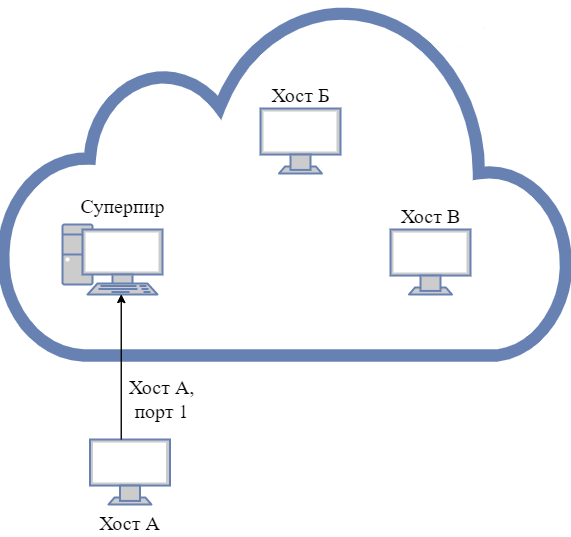
\includegraphics[width=0.57\textwidth]{IPPort1.png}
    \caption{Отправка информации хоста А о себе суперпиру}
    \label{IPPort1.png}
\end{figure}

\begin{figure}[H]
    \centering
    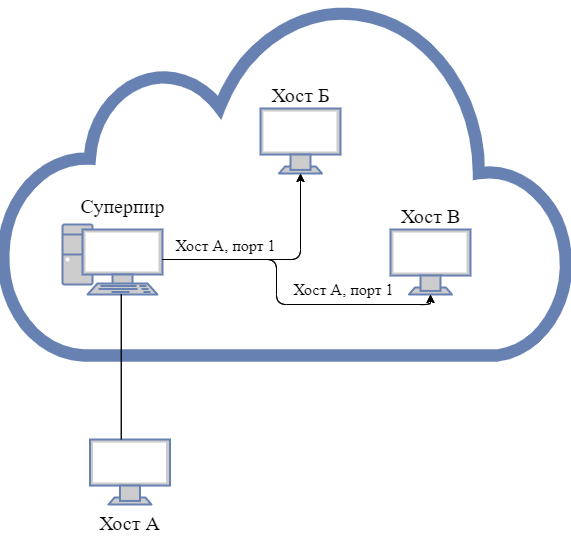
\includegraphics[width=0.57\textwidth]{IPPort2.png}
    \caption{Суперпир распространяет информацию о хосте А остальной части сети}
    \label{IPPort2.png}
\end{figure}

По существу, пара IP-адрес и порт "--- идентификатор нового хоста, который другие пиры должны использовать для подключения к нему. Когда P2P-хост инициирует TCP или UDP соединение с хостом А, порт назначения будет портом, который прослушивает хост А, а порт источника будет случайным, выбранным клиентом. 

Обычно пиры поддерживают не более одного TCP соединения с каждым другим пиром, но, как описано ранее, можно быть ещё один UDP поток. Итак, множественные соединения между пирами это редкое явление. Рассмотрим случай, если, например, 20 пиров подключатся к хосту А. Каждый из них выберет временный порт источника и подключится к объявленному порту, который прослушивает хост А. Таким образом, объявленная пара IP-адреса и порта хоста А будет связана с 20 различным IP-адресами и 20 различным портами. Таким образом, для пары хоста А количество различных IP-адресов и различных портов, используемых для подключения к нему, будет равно. Рисунок \ref{IPPort3.png} иллюстрирует данный случай.

\begin{figure}[H]
    \centering
    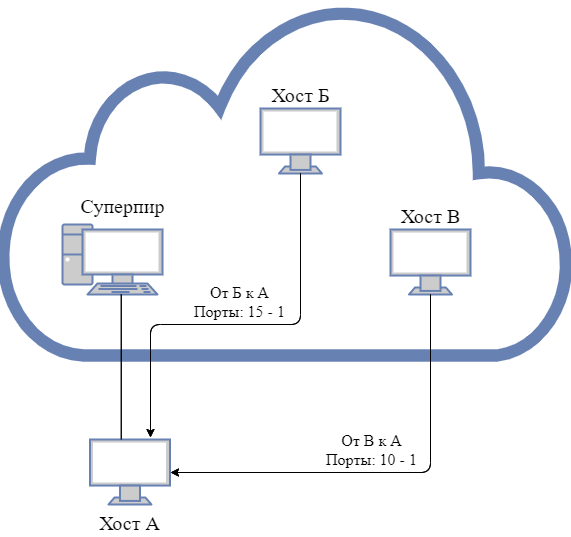
\includegraphics[width=0.57\textwidth]{IPPort3.png}
    \caption{К хосту А подключены хосты Б и В с 2 разными IP и 2 разными портами}
    \label{IPPort3.png}
\end{figure}

С другой стороны, рассмотрим случай, когда используется сеть с архитектурой клиент-сервер, пусть это будет веб-сервер. Как и в случае с P2P, каждый хост подключается к заранее определённой паре, например, IP-адрес веб-сервера и 80 порт. Однако хост, подключающийся к веб-серверу обычно инициирует несколько одновременных соединений, например, для параллельной загрузки. Тогда веб-трафик будет иметь более высокое, по сравнению с P2P-трафиком, соотношение числа отдельных портов к числу отдельных IP-адресов.

В работе \cite{blinc} приводятся графики (рисунок \ref{IPPort4.jpg}) зависимости между количеством IP-адресов назначения и портов назначения для веб- и P2P-приложений. В веб-случае большинство точек концентрируется выше диагонали, представляя параллельные соединения в основном одновременных загрузок веб-объектов. Напротив, в P2P-случае большинство точек группируется ближе к диагонали, либо немного ниже (что характерно для случаев, когда номер порта постоянен).

\begin{figure}[H]
    \centering
    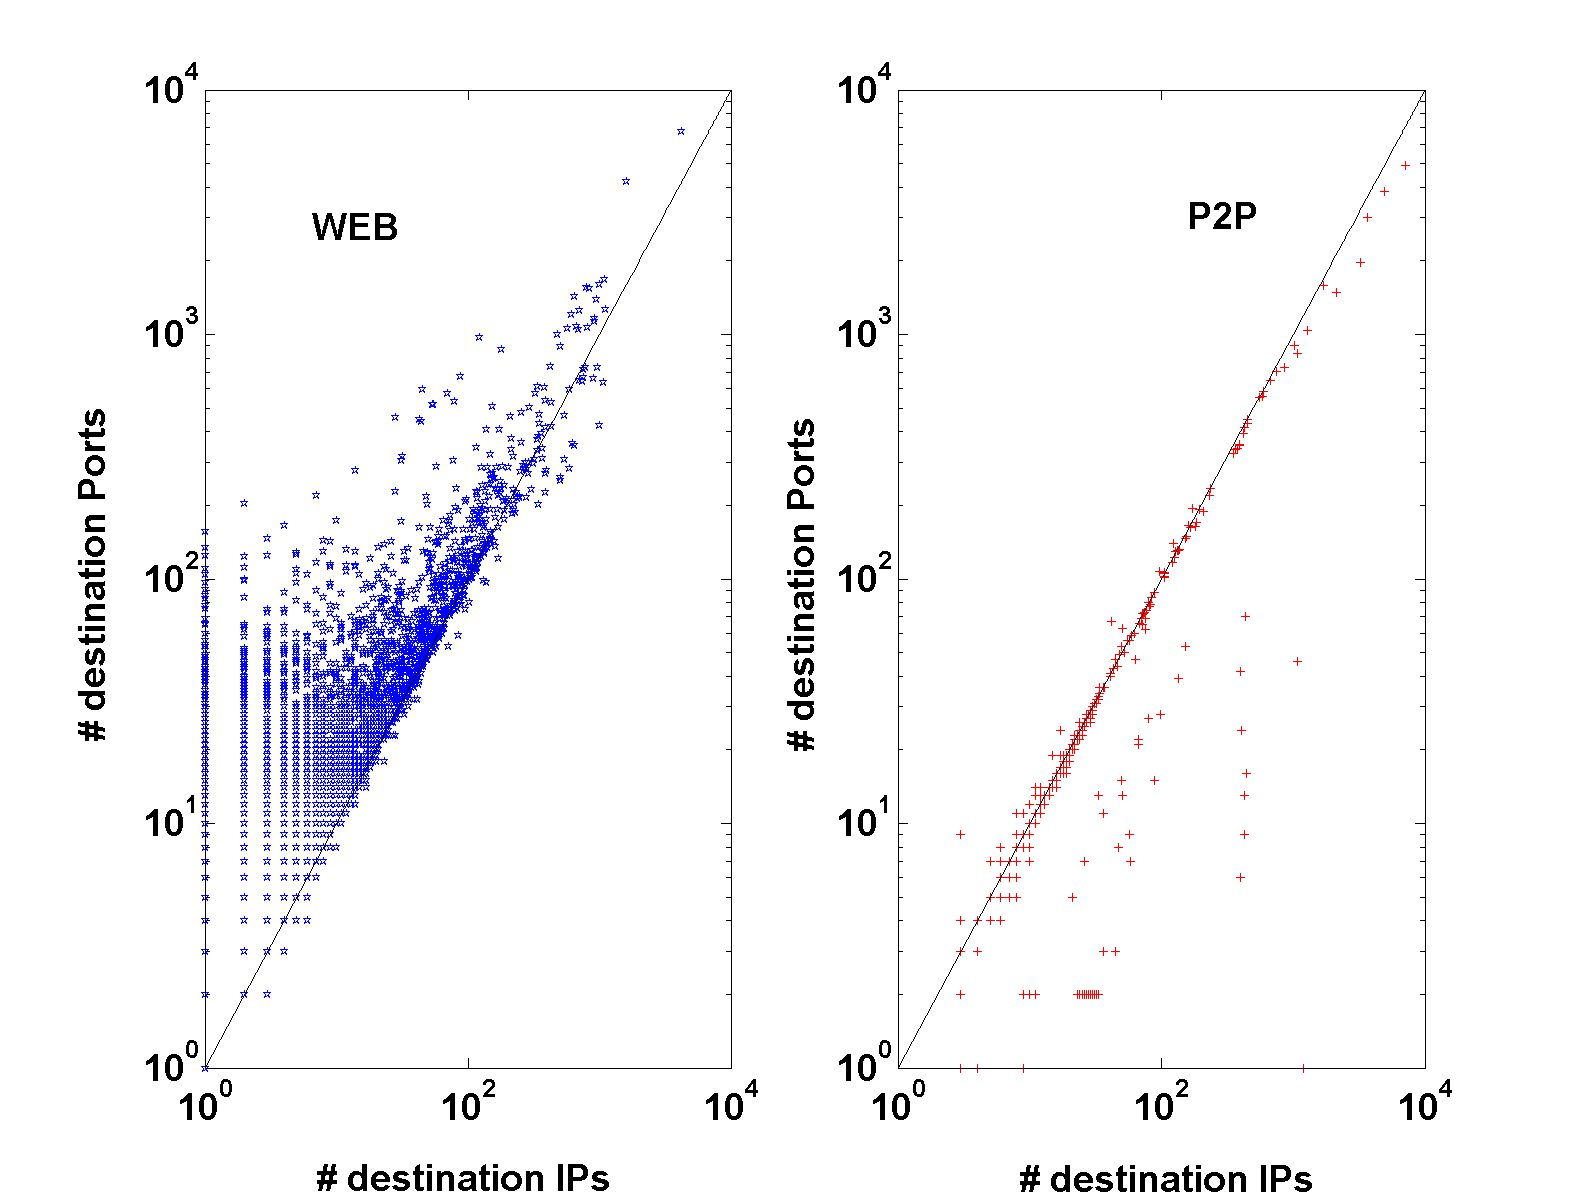
\includegraphics[width=0.75\textwidth]{IPPort4.jpg}
    \caption{}
    \label{IPPort4.jpg}
\end{figure}

Таким образом, если для пары \{IP, Port\} множество адресов источников содержит больше двух элементов и разница между длинами этого множества и множества портов источников меньше 2 (или меньше 10, если один из портов относится к известным P2P-портам), то пара заносится в список адресов данной эвристики. Если же разница больше 10, то пара заносится в список адресов-исключений. 

\subsection{Обнаружение BitTorrent}
В работе \cite{BitTorrent} предложен алгоритм, который основывается на четырёх критериях.

\subsubsection{Подключенные IP-адреса}
Первый критерий основан на IP/Port-эвристике. Хосты BitTorrent всегда подключены ко многим IP-адресам.
Под подключенными IP-адресами понимается, что они передали друг другу хотя бы
по одному TCP-пакету. В BitTorrent это может быть необходимо для подключения к раздаче и передачи особенных
сообщений (choke, have, keepalive). Причём каждый пир (участник) пытается поддерживать не менее 20 пиров, следовательно,
каждый пир периодически отправляет несколько TCP-пакетов на один и тот же набор IP-адресов.

\subsubsection{Передача данных}
BitTorrent разбивает исходные файлы на небольшие части, поэтому пользователи могут скачивать разные файлы
от разных пользователей. Это можно определить по значимому соотношению активных передач. Под активной передачей
подразумевается хотя бы 5 больших TCP-пакетов, т.е. размер пакета должен быть примерно равен \textit{MTU} (максимальная единица передачи). В Ethernet это около 1500 байт. Передача пакетов максимального размера необходима для того, 
чтобы их количество было минимальным для передачи файла.

Однако пиры BitTorrent не всегда одновременно обмениваются данными между собой. 
Это связано с \textit{алгоритмом дросселирования} (\textit{choke}). Этот алгоритм выбирает соседей, которым будут раздаваться или с которых будут скачиваться файлы. В любой момент времени пир загружает данные не более, чем 
с 4 пиров, которые обеспечивают самую высокую скорость загрузки. % там ещё предложение есть
 
\subsubsection{Двусторонняя передача данных}
Процесс выбора в алгоритме дросселирования приводит к двусторонней передаче данных. В отличие от BitTorrent, другие 
интернет-приложения обычно работают по схеме клиент-сервер, поэтому данные передаются только в одном направлении в 
определённый промежуток времени. Кроме того, в других протоколах P2P-обмена между элементами нет взаимного обмена,
который заложен в алгоритме дросселирования. Пирам в этих протоколах не нужно загружать свои фрагменты другим пирам,
с которых они скачивают данные. 

\subsubsection{Изменение отношений}
В алгоритме дросселирования все пиры в наборе сортируются каждые 10 секунд в порядке убывания скорости загрузки данных.
После сортировки локальный пир будет раздавать данные только первым четырём пирам в отсортированном списке.
Учитывая, что скорость передачи довольно динамична, выбранные пиры будут часто меняться. Таким образом, пара пиров
может активно передавать данные друг другу, но потом внезапно может стать неактивной. В результате хост BitTorrent может
быть идентифицирован по значимому соотношению изменений IP-отношений к активным передачам.

\subsubsection{Алгоритм}
На основании четырёх критериев создаются специальные метрики, которые рассчитываются каждые 30 секунд
и сравниваются с пороговым значением, чтобы определить, является ли хост пиром BitTorrent. 
%В данном алгоритме обрабатываются только TCP-пакеты. 

% \subsubsection*{Подключения}
\begin{enumerate}
    \item \textbf{Подключения}. Подсчитывается число $C$ "--- количество пиров, которые общались с хостом. Если это количество будет больше или равно порогу $C_{\text{порог.}}$, то хост будет идентифицирован как BitTorrent-хост.
    \[ C \geq C_{\text{порог.}} \]
    
    \item \textbf{Коэффициент активной передачи}. Коэффициент активной передачи хоста $R_{AT}$ "--- отношение числа активных подключений $AT$ к общему числу подключений $C$.
    Если этот коэффициент больше или равен пороговому $R_{AT\text{порог.}}$, то хост будет идентифицирован как BitTorrent-хост.
    \[ R_{AT} \geq R_{AT\text{порог.}}, \]
    где $R_{AT} = \frac{AT}{C}$.

    \item \textbf{Двусторонние передачи данных}. Измеряется количество подключений $BiAT$, по которым одновременно принимаются и отправляются данные. 
    Если это число больше или равно пороговому $BiAT_{\text{порог.}}$, то хост будет идентифицирован как BitTorrent-хост.
    \[ BiAT \geq BiAT_{\text{порог.}} \]

    \item \textbf{Коэффициент изменений отношений}. Коэффициент изменений отношений $R_{RC}$ "--- отношение числа изменений отношений $RC$ к числу активных передач $AT$.
    Если этот коэффициент больше или равен пороговому $R_{RC\text{порог.}}$, то хост будет идентифицирован как BitTorrent-хост.
    \[ R_{RC} \geq R_{RC\text{порог.}}, \]
    где $R_{RC} = \frac{RC}{AT}$.
\end{enumerate}

В качестве пороговых в программе используются следующие значения:
\begin{itemize}
    \item $C_{\text{порог.}} = 20$
    \item $R_{AT\text{порог.}} = 0.35$
    \item $BiAT_{\text{порог.}} = 5$
    \item $R_{RC\text{порог.}} = 0.5$
\end{itemize}

Данные значения являются наиболее оптимальными. Метрики <<коэффициент активной передачи>> и <<коэффициент изменений отношений>> сравниваются с пороговыми при условии, что $C$ (число подключений) больше или равно половины своего порогового значения $C_{\text{порог.}}$, то есть 10. 


\subsection{Исключения}
Чтобы снизить количество ложных срабатываний, необходимо учитывать протоколы, поведение которых может быть схожим с поведением P2P-протоколов. Стандартные сетевые протоколы обычно имеют стандартные номера портов, что очень удобно для фильтрации трафика. В то же время, для некоторых приложений всё же необходимо использовать иные подходы.

\subsubsection{Почта}
Поведение почтовых протоколов, таких как SMTP и POP, может вызвать ложное срабатывание, поскольку оно похоже на IP/Port-эвристику. Почтовые серверы возможно идентифицировать на основе использования ими портов 25 для SMTP, 110 для POP или 113 для сервиса аутентификации, который обычно используется почтовыми серверами, а также на основе наличия различных потоков в течение некоторого временного интервала, которые используют порт 25 как для порта источника, так и для порта назначения.

Таблица \ref{table:mail} иллюстрирует характерное поведение почтовых серверов:

\begin{table}[H]
    \caption{Пример почтового TCP трафика}
    \label{table:mail}
    \begin{center}
    {\small
    \begin{tabular}{|c|c|c|c|}
        \hline
    IP-адрес источника & IP-адрес назначения & Порт источника & Порт назначения \\ \hline
    238.30.35.43       &   115.78.57.213     & 25             & 3267 \\ \hline
    238.30.35.43       &    238.45.242.104   & 25             & 25 \\ \hline
    238.30.35.43       &    0.32.132.109     & 22092          & 50827 \\ \hline
    238.30.35.43       &    71.199.74.68     & 25             & 25 \\ \hline
    238.30.35.43       &    4.87.3.29        & 21961          & 25 \\ \hline
    238.30.35.43       &     4.87.3.29       & 22016          & 25 \\ \hline
    238.30.35.43       &     4.170.125.67    & 25             & 3301\\ \hline
    238.30.35.43       &     5.173.60.126    & 22066          & 25 \\ \hline
    238.30.35.43       &     5.173.60.126    & 22067          & 25 \\ \hline
    238.30.35.43       &     227.186.155.214 & 22265          & 25 \\ \hline
    238.30.35.43       &    227.186.155.214  & 22266          & 25\\ \hline
    238.30.35.43       &     5.170.237.207   & 25             & 3872 \\ \hline
    \end{tabular}
    }
    \end{center}
\end{table}

В этом примере показаны потоки для IP-адреса 238.30.35.43, где порт 25 является портом источника в одних потоках и назначения в других. Такое поведение характерно для почтовых серверов, которые инициируют подключения к другим почтовым серверам для распространения сообщений электронной почты. Для выявления такой модели отслеживается набор номеров портов назначения для каждого IP-адреса, для которого существует пара-источник \{IP, 25\}. Если этот набор номеров портов назначения также содержит порт 25, то этот IP считается за почтовый сервер, и все его потоки классифицируются как не P2P. Аналогично для набора портов источника IP, для которого существует пара-назначение \{IP, 25\}. В приведённом выше примере для пары \{238.30.35.43, 25\} набор портов назначения: 3267, 25, 50827, 3301, 3872. Так как в этом наборе есть порт 25, то из этого следует вывод, что данный IP-адрес относится к почтовому серверу и все его потоки будут считать не P2P.

\subsubsection{DNS}
Протокол DNS, как и почтовые протоколы, может быть ложно принят за P2P из-за IP/Port-эвристики, хотя DNS легче идентифицировать, поскольку обычно порты источника и назначения равны 53. 

Таким образом, если найдётся пара \{IP, 53\}, которая будет либо источником, либо назначением, то все потоки, содержащие данный IP-адрес, будут считаться как не P2P. Заметим, что при этом потоки,
содержащие обращения к DNS-службе со стороны участников P2P-обмена, также считаются
не P2P. Однако P2P-клиенты имеют небольшое количество обращений к DNS-службе, так
как получают нужную информацию друг от друга.

\subsubsection{Игры и вредоносные программы}
Игры и вредоносные программы (malware) характеризуются однотипными потоками,
имеющими одну и ту же длину или небольшой разброс средних размеров пакетов в потоке. Для исключения такого взаимодействия сохраняется соответствующая информация и проводится проверка. Однако такая проверка трудно реализуема, поскольку размеры пакетов будут зависеть от каждой конкретной игры или вредоносной программы. В работе \cite{algorithm} выдвигается предположение, что множество длин не будет превышать, например, трёх. Хотя на практике множество длин обычно намного больше, чем три. 

Например, на рисунках \ref{wt} и \ref{dota2} изображены гистограммы, построенные на основе перехваченного сетевого трафика двух многопользовательских игр: \textit{War Thunder} и \textit{Dota 2} в течение одной игровой сессии. Трафик обоих игр был определён реализованной в данной работе программой как P2P по IP/Port-эвристике. 

Здесь каждому столбцу по горизонтали соответствует диапазон размеров пакетов в байтах и по вертикали среднее их количество по диапазону. Так, в War Thunder большая часть пакетов имеет размер 18 байт, в то время как в Dota 2 "--- около 150 байт. 

\begin{figure}[H]
    \centering
    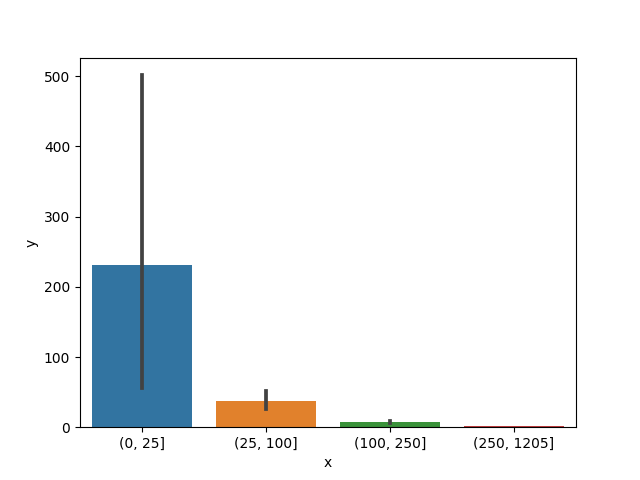
\includegraphics[width=0.75\textwidth]{warthunder.png}
    \caption{Графическое представление среднего количества пакетов различных диапазонов их размеров в игре War Thunder}
    \label{wt}
\end{figure}

\begin{figure}[H]
    \centering
    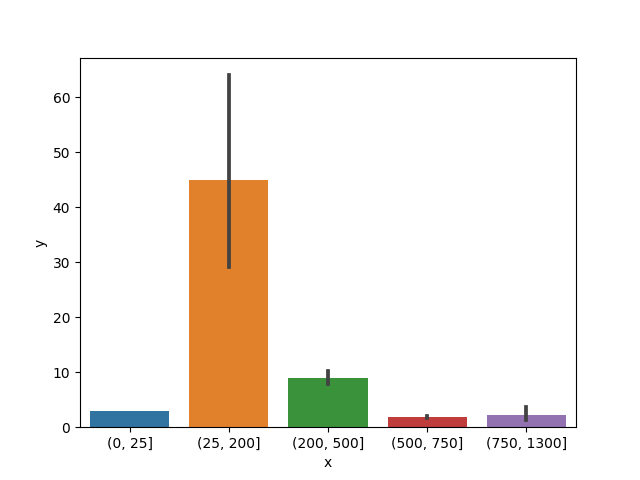
\includegraphics[width=0.75\textwidth]{dota2.png}
    \caption{Графическое представление среднего количества пакетов различных диапазонов их размеров в игре Dota 2}
    \label{dota2}
\end{figure}

Хорошо видно, что игровой трафик обычно характеризуется отправкой небольших пакетов. Но могут встречаться и большие пакеты, например, при передаче больших объемов данных или при обмене файлами внутри игрового приложения. Тем не менее, только лишь по данному признаку нельзя точно определить игровой трафик, так как и другие сетевые приложения могут иметь данный признак. Для большей точности, предположительно, стоит дополнительно использовать определение по номерам портов и анализ полезной нагрузки пакетов. 

\subsubsection{Сканирование}
Если адрес назначения \{IP, Port\} подвергается распределенному сканированию или атаке со
стороны множества адресов, то обычно ответы от пары \{IP, Port\} отсутствуют или их крайне мало. В таком случае, если данная пара не была определена ранее как P2P, то она считается как не P2P, несмотря на верность IP/Port-эвристики. В таком случае говорят, что верна эвристика сканирования.

\subsubsection{Известные порты}
Наконец, если в потоке порт источника и порт назначения совпадают, и оба меньше или равны 500, то такой поток считается не P2P. Подобное поведение нехарактерно для P2P, но характерно для ряда легальных взаимодействий, например, для сервисов NTP (порт 123) или DNS (порт 53). 

\section{Обнаружение P2P трафика при помощи анализа полезной нагрузки}
% мб получше написать
Анализ полезной нагрузки пакетов может оказаться достаточно трудоёмким или вовсе не реализуемым в конкретный временной промежуток процессом, поскольку существует множество факторов, ограничивающих исследование передаваемых данных. Во-первых, всё большее число приложений и протоколов используют шифрование и TLS (transport layer security) при передаче пакетов по сети. По этой причине сопоставить некоторые шаблонные строки с информацией, обнаруженной внутри перехваченного пакета, становится невозможно. Во-вторых, сигнатуры каждого конкретного приложения могут меняться, поэтому их базу придётся регулярно обновлять. В-третьих, некоторые протоколы, в особенности проприетарные, например, протокол Skype, используют обфускацию данных в пакете, что дополнительно усложняет их анализ \cite{skype_obf}. 

Тем не менее, некоторые современные протоколы могут передавать часть информации в открытом, незашифрованном виде. Если обнаружить момент передачи такой информации и идентифицировать протокол, с помощью которого эти данные были переданы, то далее в определённый временной промежуток можно считать пару адресов, участвующих в этой передаче, за участников или пользователей некой сети (в данной работе интерес представляют именно P2P-сети).

\subsection{Обнаружение BitTorrent}
Первым сообщением, которое обязан передать клиент перед началом соединения, является handshake (рукопожатие).
Формат рукопожатия следующий \cite{bittorrent_sp}:
\begin{itemize}
    \item \textbf{pstrlen}: длина имени протокола;
    \item \textbf{pstr}: имя протокола;
    \item \textbf{reserved}: 8 резервных байт;
    \item \textbf{info_hash}: 20-байтовый SHA1 хэш информационного ключа файла \\ \texttt{Metainfo};
    \item \textbf{peer_id}: 20-байтовая строка, представляющая собой уникальный номер клиента.
\end{itemize}

Именно handshake пакеты представляют интерес при обнаружении \\ BitTorrent, поскольку первые два заголовка передаются в открытом виде. На основе этих заголовков и формируются условия, при которых пакет относится к BitTorrent:
\begin{enumerate}
    \item Минимальная длина полезной нагрузки пакета 20 байт.
    \item Байт со значением 19.
    \item Следующая за ним строка <<BitTorrent protocol>>.
\end{enumerate}

В шестнадцатиричном формате заголовки \textit{pstrlen} и \textit{pstr} будут выглядеть как <<\texttt{13 42 69 74 54 6f 72 72 65 6e 74 20 70 72 6f 74 6f 63 6f 6c}>>.

При выполнении всех перечисленных условий считается, что пара адресов (вместе с номерами портов) взаимодействует при помощи BitTorrent, поэтому они отмечаются как P2P. В дальнейшем, все проходящие пакеты между этой парой адресов считаются как пакеты BitTorrent.

\subsection{Обнаружение Bitcoin}
Сеть Bitcoin использует специальный порт для обмена данными между узлами "--- 8333 для протокола TCP и 8334 для протокола UDP. При этом, обмен данными в сети Bitcoin шифруется, что затрудняет идентификацию трафика.

Однако Bitcoin использует специфичные сообщения (назовём их словами Bitcoin) \cite{bitcoin_sp}: 
\texttt{version, verack, addr, inv, getdata, notfound, getblocks, getheaders, tx,  
block, headers, getaddr, mempool, \\ checkorder, submitorder, reply, ping, pong, reject, 
filterload, \\ filteradd, filterclear, merkleblock, alert, sendheaders, \\ feefilter,
sendcmpct, cmpctlblock, getblocktxn, blocktxn, Satoshi}.

Исходя из данных особенностей, пара адресов (вместе с номерами портов) считается участниками Bitcoin-сети, если выполняются следующие условия:
\begin{enumerate}
    \item Минимальная длина полезной нагрузки пакета 20 байт.
    \item Порт источника или назначения равен 8333 или 8334.
    \item В пакете содержится любое из слов Bitcoin.
\end{enumerate}

Выполнение одновременно 2 и 3 условий необходимо для того, чтобы, насколько это возможно, исключить те случаи, когда иные приложения используют порты Bitcoin или те же самые слова. Например, слово <<version>> может встречаться в HTTP, FTP, Git, SVN и так далее.

\section{Описание программы}
В данной работе был разработан \textbf{сниффер} "--- анализатор сетевого трафика. Использованный язык программирования "--- Python.
Программа выводит на экран информацию о перехваченных пакетах таких сетевых протоколов как \textit{IPv4}, \textit{TCP} и \textit{UDP} и анализирует перехваченный трафик на его принадлежность к P2P-сетям, а также определяет часть P2P-протоколов и приложений, например, BitTorrent, Bitcoin и Skype. Сканирование производится каждые 75 мс.
Дополнительно последний вывод программы сохраняется в текстовые файлы.

При запуске необходимо выбрать прослушиваемый сетевой интерфейс из предложенного списка:
\begin{figure}[H]
    \centering
    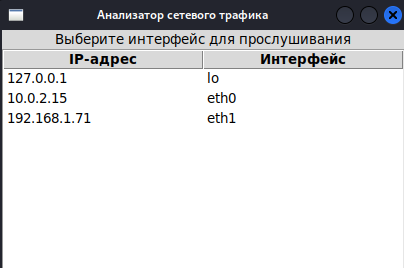
\includegraphics[width=0.5\textwidth]{ifaces.png}
    \caption{Выбор сетевого интерфейса при старте программы}
\end{figure}
Для указанного сетевого интерфейса программа включает неразборчивый режим.

Далее происходит перехват TCP/UDP трафика и вывод информации о нём в левой части окна. В правой части расположены списки адресов тех узлов, которые программа определила как участников P2P-сети. Каждому списку соответствует конкретный метод обнаружения. В правом нижнем списке с подписью <<Пересечение методов>> выводятся адреса, которые были обнаружены хотя бы двумя различными методами одновременно.

\begin{figure}[H]
    \centering
    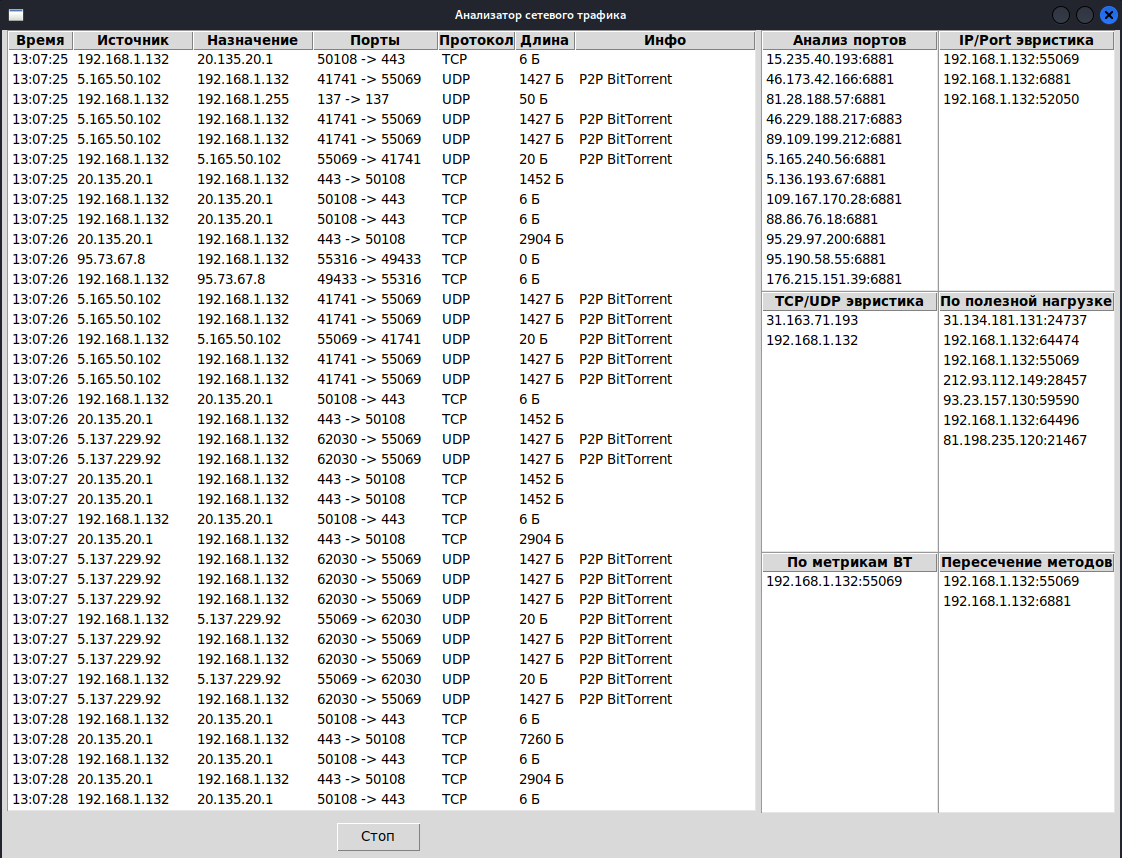
\includegraphics[width=1\textwidth]{window.png}
    \caption{Основное окно программы}
\end{figure}

Для обработки исключений используется следующий алгоритм: для каждой пары адресов \{src_ip, src_port\} $\to$ \{dest_ip, dest_port\} проверяется, если один из портов находится в списке портов-исключений или порт источника src_port равен порту назначения dest_port, и они оба меньше или равны 500, то обе пары адресов заносятся в список адресов-исключений. Далее при вызове любого из методов обнаружения P2P-трафика сначала проверяется, не является ли пара исключением. Если нет, то применяется сам метод.

Метод анализа портов и полезной нагрузки вызываются для каждого нового пакета. Проверка TCP/UDP- и IP/Port-эвристики вызывается каждые 15 секунд. Сравнение метрик BitTorrent проводится каждые 30 секунд.

Определение P2P-протоколов выполняется при помощи анализа портов, полезной нагрузки и метода сравнения метрик BitTorrent. Увидеть результат определения можно в левой части окна программы в столбце <<Инфо>>.

\subsection{Тестирование}
Тестирование проводилось при следующих условиях: программа запущена на виртуальной машине под операционной системой Linux, дистрибутив Kali в программе VirtualBox. Хостовая машина под Windows 10 подключена к виртуальной через сетевой мост с включенным неразборчивым режимом. Все приложения запускаются на хостовой машине, а программа, запущенная на виртуальной машине, перехватывает сетевой трафик этих приложений.

IP-адрес хостовой машины: 192.168.1.132, виртуальной "--- 192.168.1.71.
\begin{figure}[H]
    \centering
    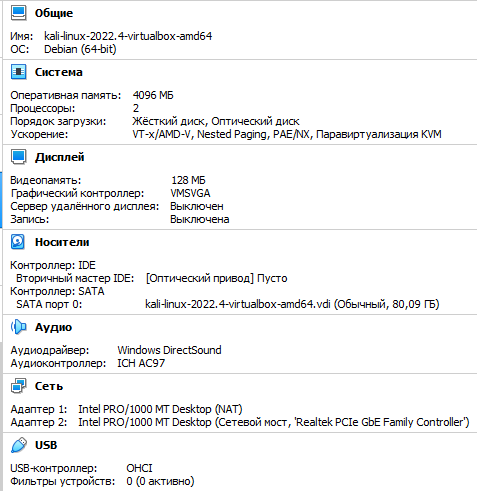
\includegraphics[width=0.6\textwidth]{vbox.png}
    \caption{Настройки виртуальной машины}
\end{figure}

С помощью монитора ресурсов <<resmon>> на Windows 10 можно просмотреть список TCP-подключений и прослушиваемые TCP/UDP порты, чтобы проверить принадлежность адреса или порта к какому-либо сетевому приложению.

Работа программы при активном веб-трафике (видео, музыка, социальные сети и загрузка файла с облака):
\begin{figure}[H]
    \centering
    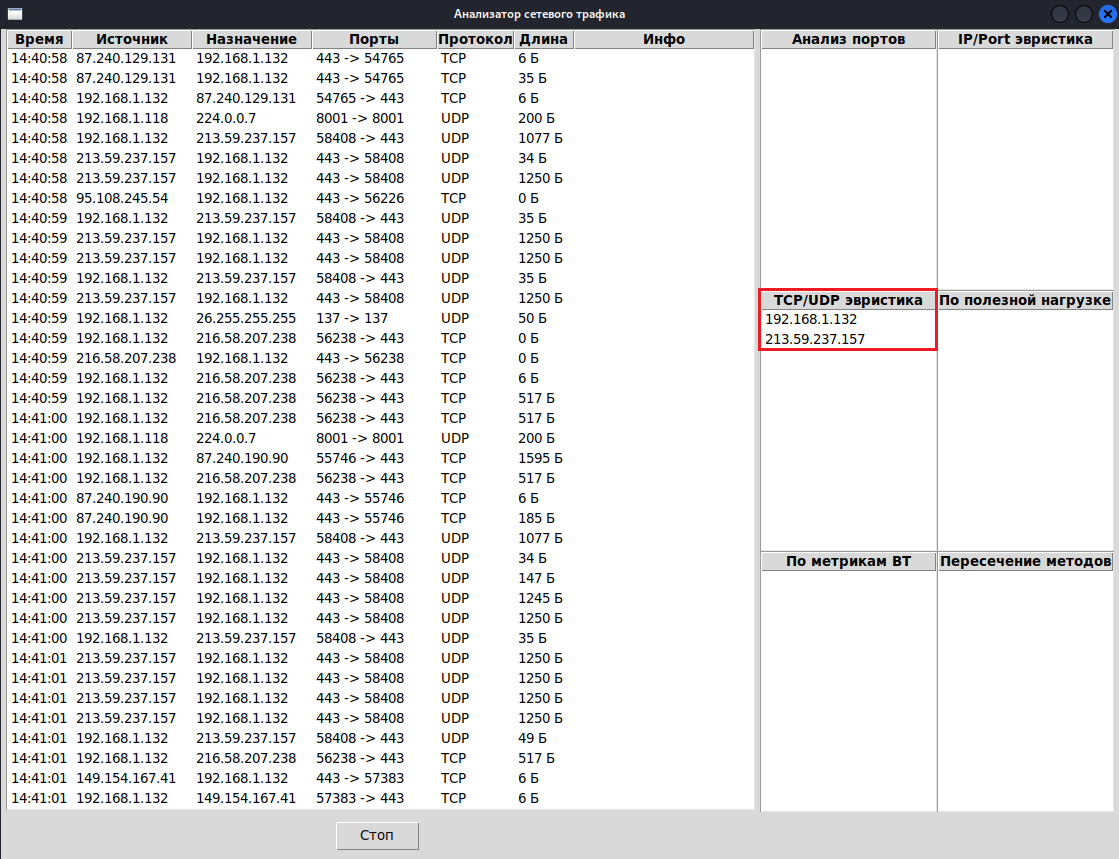
\includegraphics[width=1\textwidth]{test1.png}
    \caption{Тестирование при активном веб-трафике}
\end{figure}

Программа определила два IP-адреса как P2P с помощью одного метода "--- TCP/UDP-эвристики. Первый адрес является адресом хостовой машины. На рисунке \ref{resmon1} можно увидеть, что второй адрес относится к браузеру, следовательно, срабатывание было ложным. 
\begin{figure}[H]
    \centering
    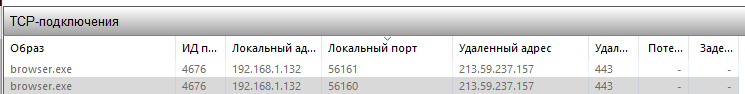
\includegraphics[width=0.85\textwidth]{test1_resmon.png}
    \caption{Информация об адресе в resmon}
    \label{resmon1}
\end{figure}

В каждом последующем тестовом запуске будет присутствовать активный веб-трафик.

Следующий запуск проводился при загрузке файла через \textmu Torrent, клиент BitTorrent:
\begin{figure}[H]
    \centering
    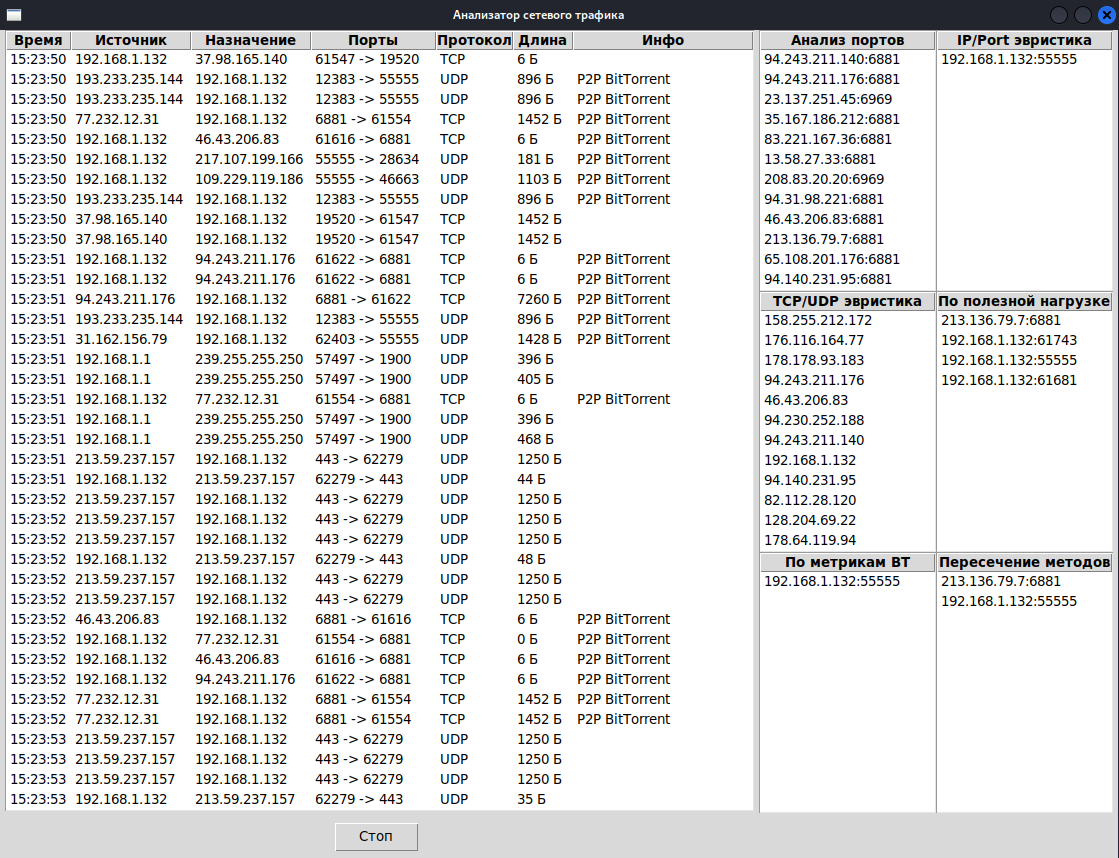
\includegraphics[width=1\textwidth]{test2.png}
    \caption{Тестирование при загрузке файла через \textmu Torrent}
\end{figure}

Видно, что было обнаружено множество адресов с помощью всех реализованных методов. В частности, адрес 192.168.1.132:55555 является адресом входящих соединений \textmu Torrent. На рисунке \ref{test2_btset} можно увидеть данную настройку. Этот адрес был помечен сразу несколькими методами: по IP/Port-эвристике, полезной нагрузке и метрикам BitTorrent. Не все пиры были обнаружены программой, однако, если сравнить результат работы программы и информацию на рисунках \ref{test2_resmon} и \ref{test2_peers}, то можно увидеть, что многие адреса всё же были определены.

Также в выводе информации о трафике появляются пометки в потоках, принадлежащих BitTorrent.

\begin{figure}[H]
    \centering
    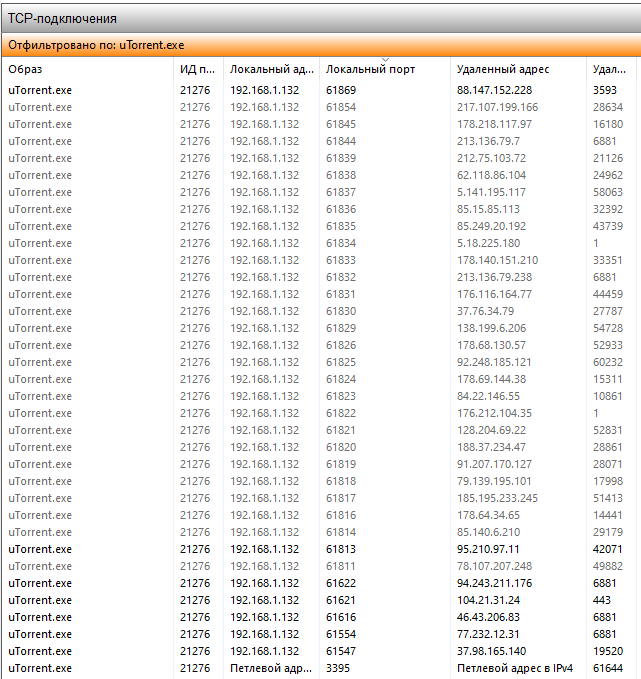
\includegraphics[width=0.9\textwidth]{test2_resmon.png}
    \caption{Информация о TCP-подключениях клиента \textmu Torrent в resmon}
    \label{test2_resmon}
\end{figure}

\begin{figure}[H]
    \centering
    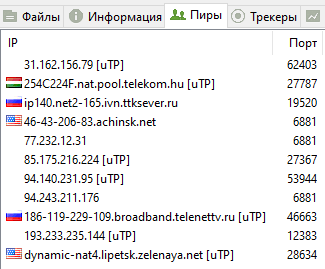
\includegraphics[width=0.45\textwidth]{test2_peers.png}
    \caption{Активные пиры клиента \textmu Torrent}
    \label{test2_peers}
\end{figure}

\begin{figure}[H]
    \centering
    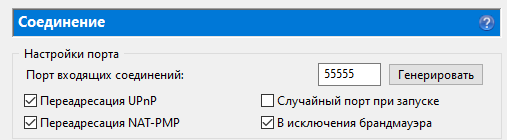
\includegraphics[width=0.65\textwidth]{test2_btset.png}
    \caption{Настройка порта входящих соединений клиента \textmu Torrent}
    \label{test2_btset}
\end{figure}

Аналогичные результаты были получены при загрузке файла с помощью браузерного BitTorrent клиента \textmu Torrent Web:
\begin{figure}[H]
    \centering
    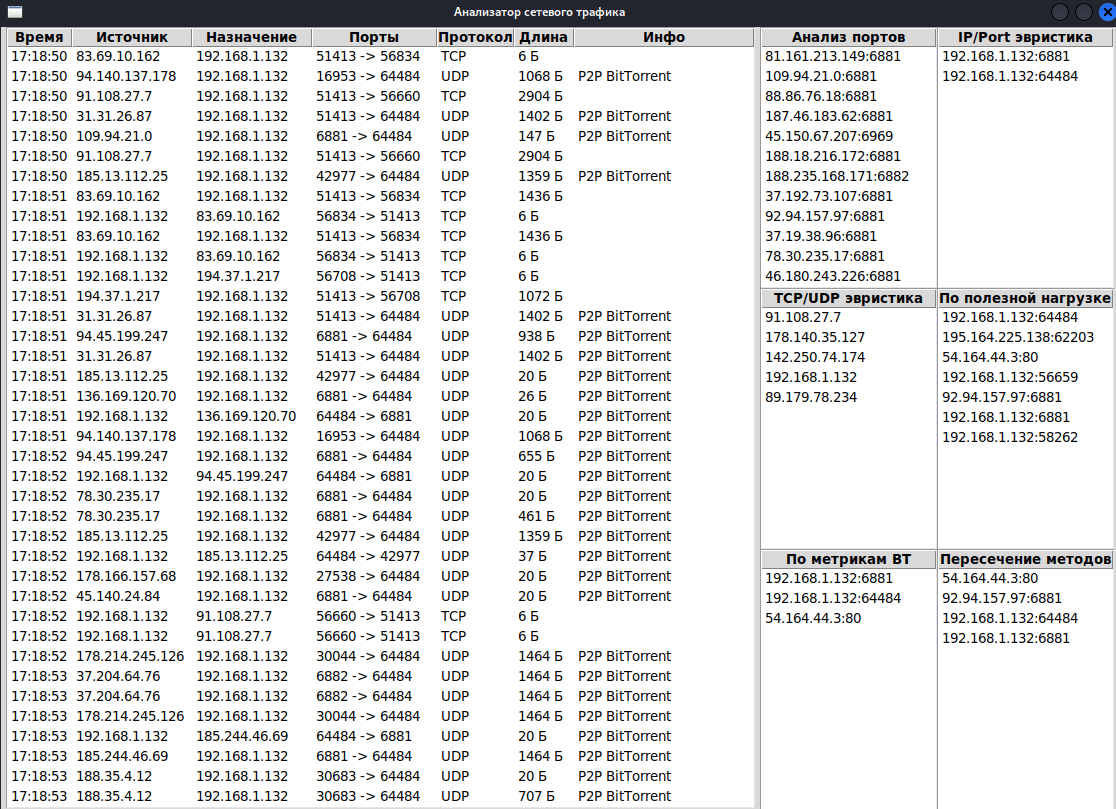
\includegraphics[width=1\textwidth]{test3.png}
    \caption{Тестирование при загрузке файла через \textmu Torrent Web}
\end{figure}

\begin{figure}[H]
    \centering
    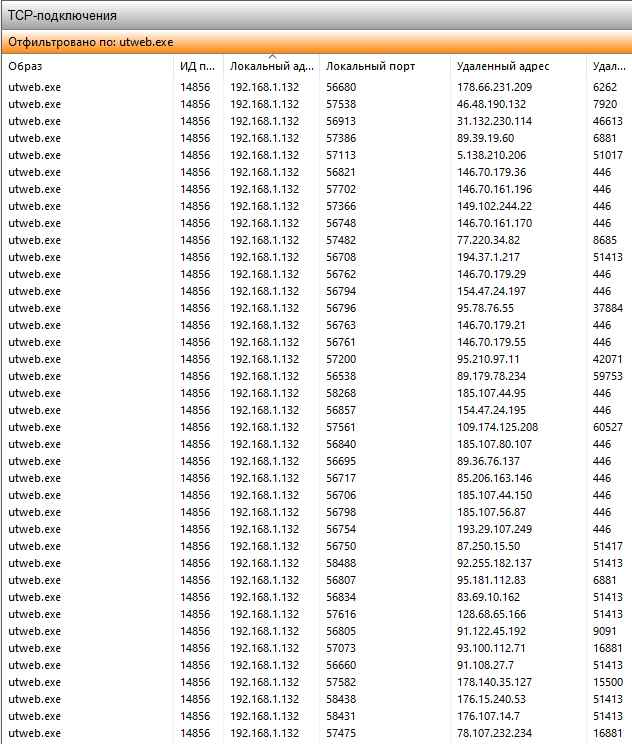
\includegraphics[width=0.9\textwidth]{test3_resmon1.png}
    \caption{Информация о TCP-подключениях клиента \textmu Torrent Web в resmon}
    \label{test3_resmon1}
\end{figure}

\begin{figure}[H]
    \centering
    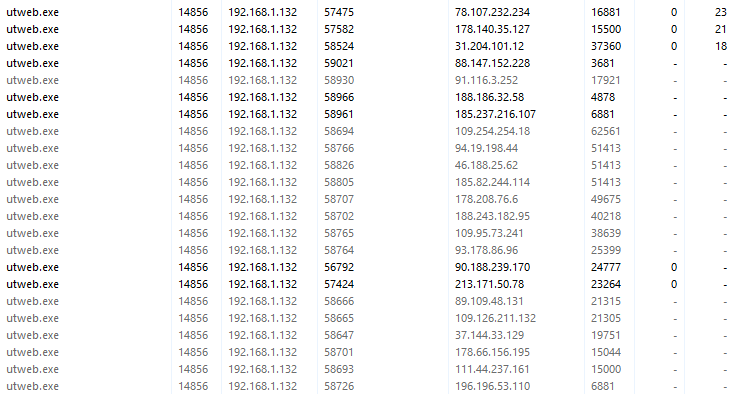
\includegraphics[width=0.9\textwidth]{test3_resmon1.2.png}
    \caption{Информация о TCP-подключениях клиента \textmu Torrent Web в resmon}
    \label{test3_resmon1.2}
\end{figure}

\begin{figure}[H]
    \centering
    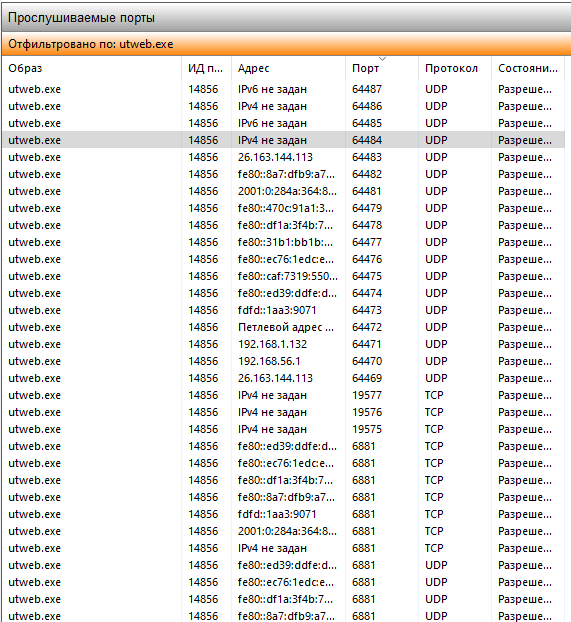
\includegraphics[width=0.8\textwidth]{test3_resmon2.png}
    \caption{Информация о прослушиваемых портах клиента \textmu Torrent Web в resmon}
    \label{test3_resmon2}
\end{figure}

Программа успешно обнаруживает работу клиента Bitcoin Core:
\begin{figure}[H]
    \centering
    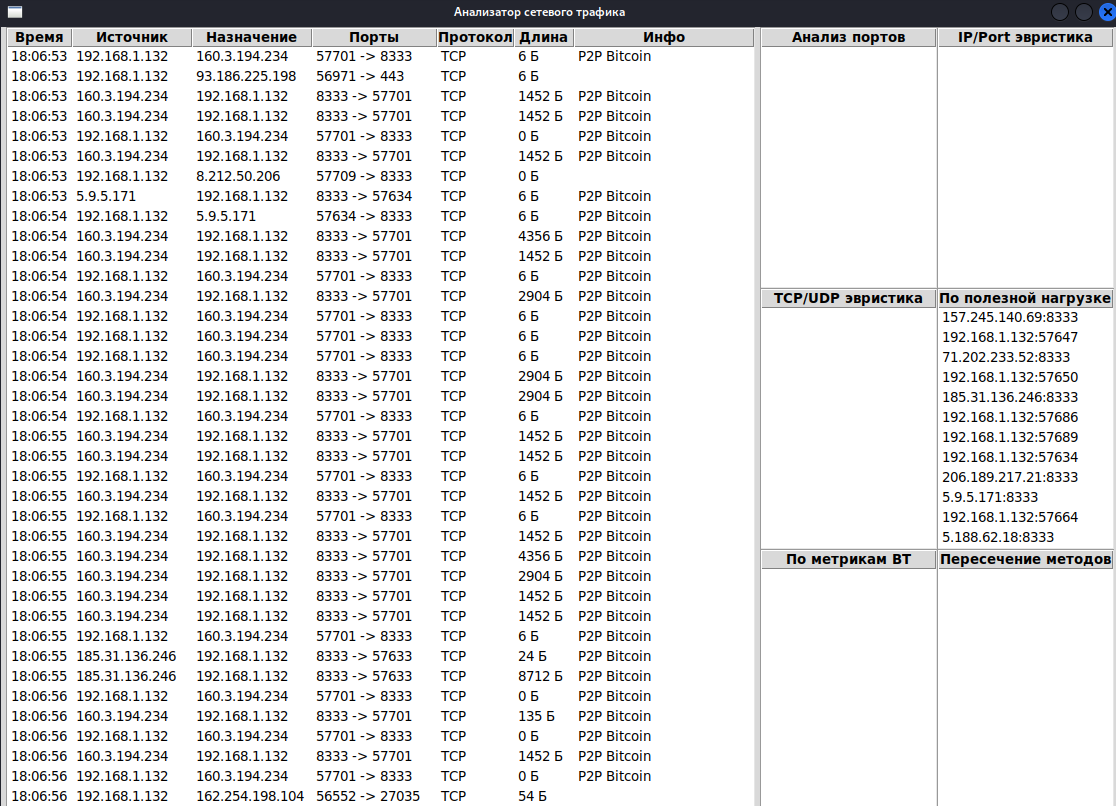
\includegraphics[width=1\textwidth]{test4.png}
    \caption{Тестирование при работе Bitcoin Core}
\end{figure}

\begin{figure}[H]
    \centering
    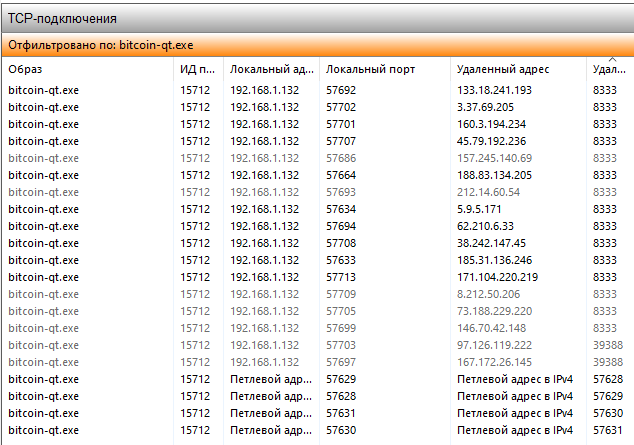
\includegraphics[width=0.9\textwidth]{test4_bc.png}
    \caption{Информация о TCP-подключениях клиента Bitcoin Core}
    \label{test4_bc}
\end{figure}

Skype успешно детектируется во время звонка при помощи анализа портов и TCP/UDP-эвристики:
\begin{figure}[H]
    \centering
    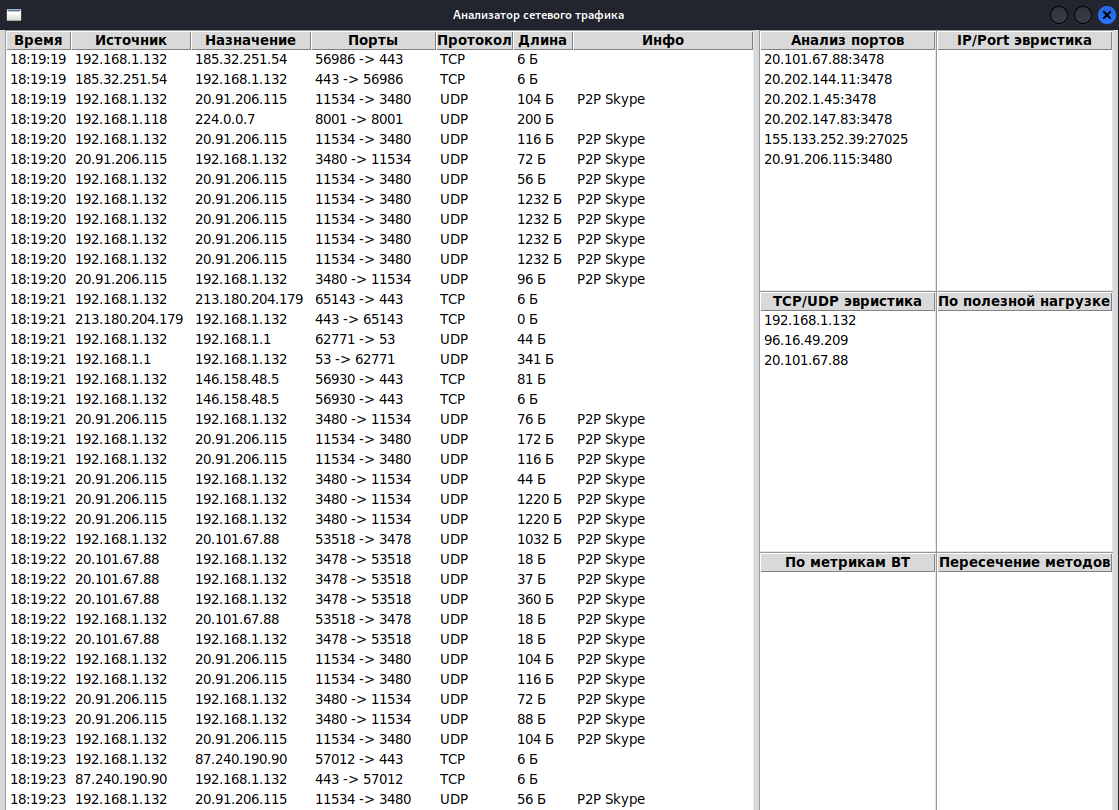
\includegraphics[width=1\textwidth]{test5.png}
    \caption{Тестирование при работе Skype}
\end{figure}

\begin{figure}[H]
    \centering
    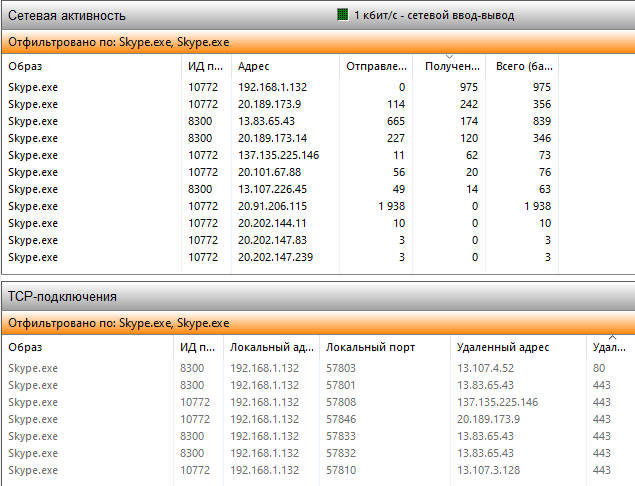
\includegraphics[width=0.8\textwidth]{test5_resmon.png}
    \caption{Информация о TCP-подключениях и прослушиваемых портах Skype}
    \label{test5_resmon}
\end{figure}

Для следующего теста была создана общая папка на хостовой машине. Доступ к ней был открыт в локальной сети. 
\begin{figure}[H]
    \centering
    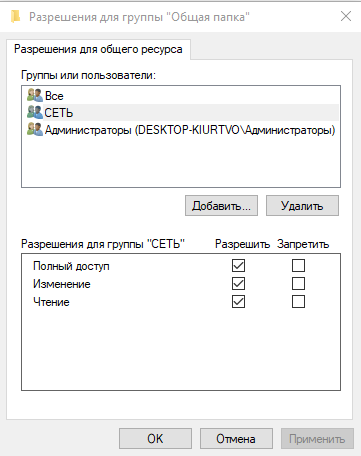
\includegraphics[width=0.45\textwidth]{Screenshot_2.png}
    \caption{Настройки доступа к папке}
\end{figure}

\begin{figure}[H]
    \centering
    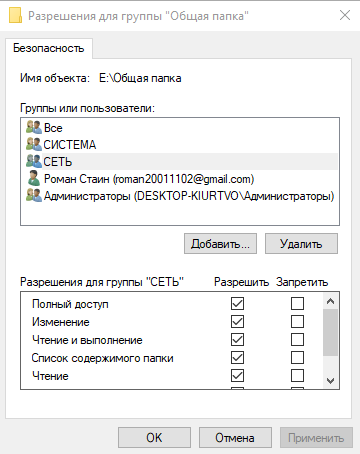
\includegraphics[width=0.45\textwidth]{Screenshot_3.png}
    \caption{Настройки безопасности папки}
\end{figure}

\begin{figure}[H]
    \centering
    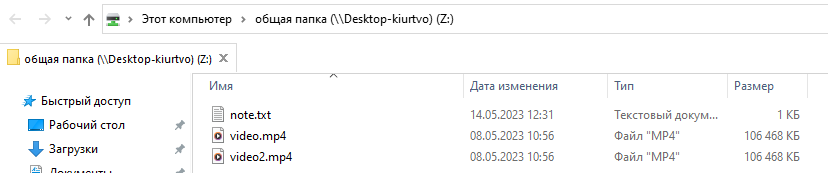
\includegraphics[width=1\textwidth]{papka2.png}
    \caption{Просмотр содержимого общей папки на хостовой машине}
\end{figure}

\begin{figure}[H]
    \centering
    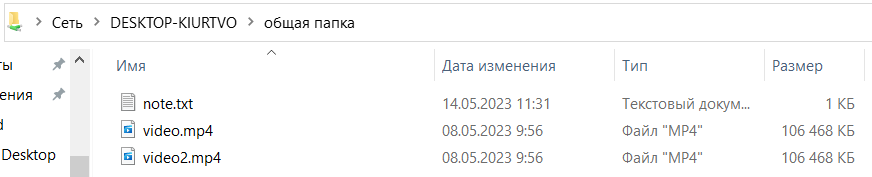
\includegraphics[width=0.9\textwidth]{papka3.png}
    \caption{Просмотр содержимого общей папки на другой машине в локальной сети}
\end{figure}

С одной машины на другую передавался видеофайл размером 103 МБ. На рисунке \ref{test7} можно увидеть, что передаются пакеты между двумя локальными адресами: 192.168.1.132 и 192.168.1.142. В итоге программа не определила данную передачу как P2P. 
\begin{figure}[H]
    \centering
    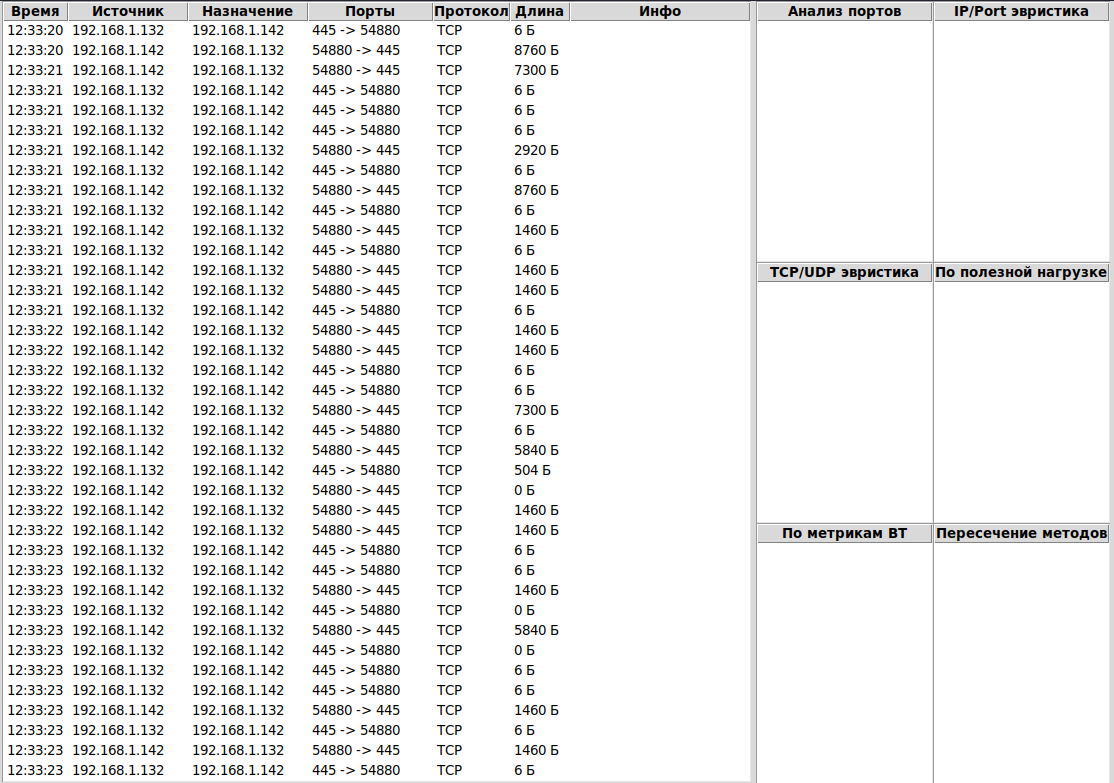
\includegraphics[width=1\textwidth]{test7.png}
    \caption{Результат работы программы}
    \label{test7}
\end{figure}

Последнее тестирование проводилось не на хостовой машине, а на виртуальной Kali Linux. Выполнение команды \texttt{apt-get update}, которая обновляет базу данных доступных пакетов, программа ложно определила как P2P с помощью метрик BitTorrent:
\begin{figure}[H]
    \centering
    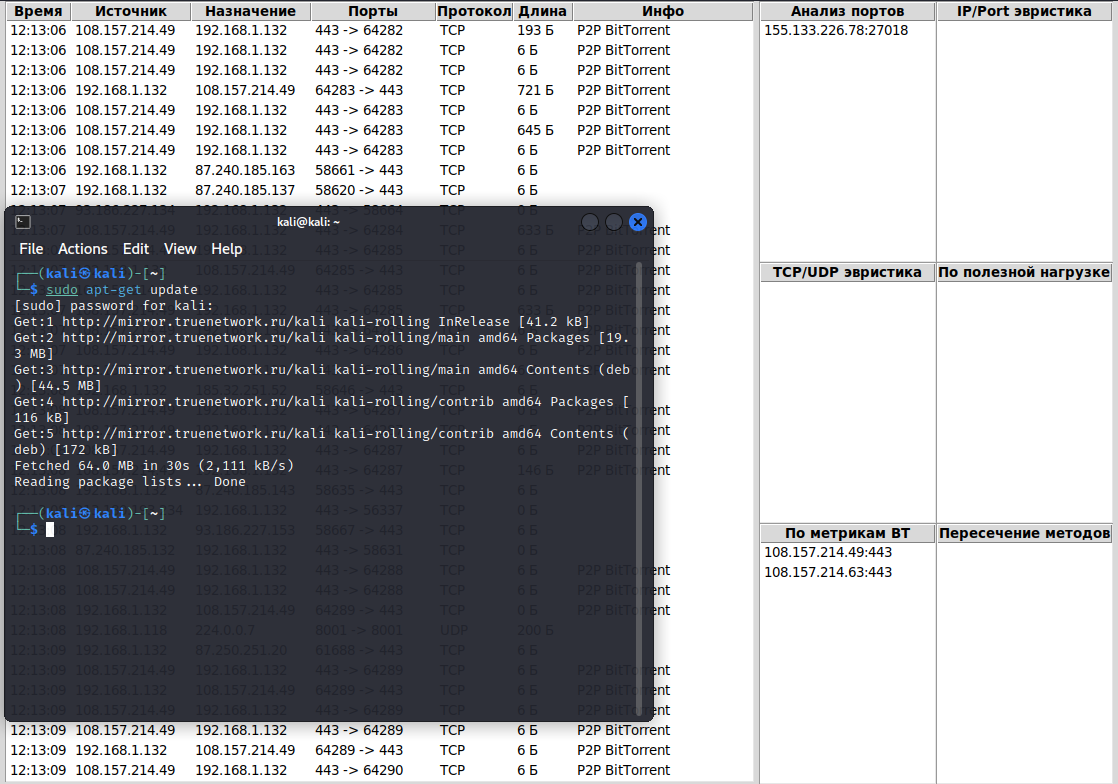
\includegraphics[width=1\textwidth]{test6.png}
    \caption{Результат работы программы}
    \label{test6}
\end{figure}

Данный метод сработал, поскольку для двух адресов, которые можно увидеть на рисунке \ref{test6}, максимальное значение метрики $C$ (количество подключений) было 51 и метрики $BiAT$ (двусторонние передачи) 38, что больше пороговых значений.

\conclusion
В данной работе были рассмотрены теоретические сведения о технологии P2P: особенности её архитектуры, применение
и способы обнаружения, которые, так или иначе, имеют некоторую степень погрешности. Вместе с тем, были приведены характерные черты такого протокола как BitTorrent, который является одним из самых распространённых среди P2P-сетей.
Поэтому обнаружение BitTorrent можно считать наиболее востребованным.

В практической части была реализована программа "--- сниффер или анализатор сетевого трафика на языке Python, которая позволяет
перехватывать TCP и UDP трафик и анализировать его на присутствие P2P-активности, а также определять некоторые протоколы и приложения. Были реализованы методы анализирования портов, обнаружения TCP/UDP- и IP/Port-эвристики, анализ полезной нагрузки для BitTorrent и Bitcoin и пороговый метод сравнения характерных метрик BitTorrent.

Таким образом, изучение P2P-сетей несомненно является актуальным, поскольку они активно используются пользователями Интернета, в следствие чего не останавливается и их развитие. Однако иногда необходимо фильтровать и блокировать P2P-трафик, поэтому необходимо также быстро развивать методы его обнаружения, которые могут устаревать со временем. P2P-протоколы меняют своё поведение, могут использовать случайные номера портов, изменять сигнатуры. Кроме того, многие другие сетевые протоколы могут иметь схожее поведение, поэтому крайне важно различать их между собой, обновлять способы исключения таких протоколов. Из-за множества подобных факторов не существует универсального способа обнаружения P2P-трафика. Тем не менее, есть необходимое количество узконаправленных методов, которые в совокупности с достаточной 
точностью могут определить P2P-активность в сети.

\bibliographystyle{gost780uv}
\inputencoding{cp1251}
\bibliography{thesis}
\inputencoding{utf8}

\appendix

    \section{Листинг \texttt{main.py}}
    \inputminted{py}{code/sniffer/main.py}

    \section{Листинг \texttt{sniffer.py}}
    \inputminted{py}{code/sniffer/sniffer.py}

\end{document}